\documentclass[12pt]{article}
%\usepackage[UTF8]{inputenc}
\usepackage[english]{babel}
\usepackage{amsmath,amssymb}
\usepackage{xcolor}
\usepackage{graphicx}
\usepackage{caption}
\usepackage{subcaption}
\usepackage{hyperref}
\usepackage{float}

\usepackage{blindtext}
\usepackage{geometry}
\geometry{
	a4paper,
	total={190mm,277mm}, % a4 is 210 x 297 mm
	left=10mm,
	top=17mm,
}

%code
\usepackage{listings}
\definecolor{codegreen}{rgb}{0,0.6,0}
\definecolor{codegray}{rgb}{0.5,0.5,0.5}
\definecolor{codepurple}{rgb}{0.58,0,0.82}
\definecolor{backcolour}{rgb}{0.95,0.95,0.92}

\lstdefinestyle{mystyle}{
	backgroundcolor=\color{backcolour},   
	commentstyle=\color{codegreen},
	keywordstyle=\color{magenta},
	numberstyle=\tiny\color{codegray},
	stringstyle=\color{codepurple},
	basicstyle=\ttfamily\footnotesize,
	breakatwhitespace=false,         
	breaklines=true,                 
	captionpos=b,                    
	keepspaces=true,                 
	numbers=left,                    
	numbersep=5pt,                  
	showspaces=false,                
	showstringspaces=false,
	showtabs=false,                  
	tabsize=2
}

\lstset{style=mystyle}

%\lstset{ 
%	upquote=true,
%	columns=fullflexible,
%	basicstyle=\ttfamily,
%	literate={*}{{\char42}}1
%	{-}{{\char45}}1
%	{\ }{{\copyablespace}}1
%}

\usepackage[space=true]{accsupp}
\newcommand{\copyablespace}{\BeginAccSupp{method=hex,unicode,ActualText=00A0}\hphantom{x}\EndAccSupp{}}

\begin{document}

%\begin{abstract}

%\end{abstract}


\section{Theory}

Any one-variable infinitely differentiable real-valued function $ f(x): A \rightarrow B $ where $A,B \subseteq \mathbb{R}$ might be expanded as an infinite power series function with parameter $ x_0 \in A $, This series function is also termed as \textbf{Taylor series} representation of $ f $ because of its procurement from the \textbf{Taylor's Theorem.}   
\begin{align}
	f(x) = T(x,x_0) &= f(x_0)+{\frac {f'(x_0)}{1!}}(x-x_0)+{\frac {f''(x_0)}{2!}}(x-x_0)^{2}+{\frac {f'''(x_0)}{3!}}(x-x_0)^{3}+\cdots \nonumber\\
	 &= \sum _{n=0}^{\infty }{\frac {f^{(n)}(x_0)}{n!}}(x-x_0)^{n} \qquad \qquad \qquad\qquad\qquad 
\end{align}

\noindent
Taylor series representation of a function with the parameter $ x_0 = 0 $ is called the \textbf{Maclaurin series}.
\begin{align}
	f(x) = T(x,0) &= \sum _{n=0}^{\infty }{\frac {f^{(n)}(0)}{n!}}(x)^{n} 
\end{align}
\\
The point on the line $ x = x_0 $ is called the center of taylor series. The value of the function and its derivatives must be known at the center and the radius of convergence of the series is determined about this point.\\[3mm]
\noindent
\textbf{Radius of Convergence of a power series}: Every power series has a radius of convergence $R$ which is the distance of its center from the nearest singularity(point of divergence).
If $R > 0$, then the power series $ \sum_{n=0}^{\infty} {c_n (x-x_0)^n}$ converges for all $ |x-a|\leq R $ and diverges for $ |x-a| > R $. If the series converges for all x, then we write $ R=\infty $. 

\noindent \\
Taylor series representation for a function of two variables $ f(x,y): \mathbb{R}^2 \rightarrow \mathbb{R} $ about $(x,y) = (x_0,y_0)$ is given by the Taylor theorem as follows,
\begin{align}
	f(x,y) = T((x,y),(x_,y_0)) = f(x_0,y_0) + f_x|_{x_0,y_0}(x-x_0) + f_y|_{x_0,y_0}(y-y_0) + + f_xx|_{x_0,y_0}(x-x_0)^2 \nonumber\\ + f_{yy}|_{x_0,y_0}(y-y_0)^2 + f_{xy}|_{x_0,y_0}(x-x_0)(y-y_0) + \cdots
\end{align}

\noindent \\
The functions $ \exp(x),\sin(x),\cos(x): \mathbb{R} \rightarrow \mathbb{R}$ are defined by the following Maclaurin series expansions.
\begin{align}
	\exp(x) &=\sum _{n=0}^{\infty }{\frac {x^n}{n!}} &\quad {\text{for all }}x\\
	\sin(x) &=\sum _{n=0}^{\infty }{\frac {(-1)^{n}}{(2n+1)!}}x^{2n+1} &\quad {\text{for all }}x\\
	\cos(x) &=\sum _{n=0}^{\infty }{\frac {(-1)^{n}}{(2n)!}}x^{2n} &\quad {\text{for all }}x
\end{align}

\section{Algorithm}
\newpage
\section{Programming}
First we defined the following functions for MySinSeries,MyCosSeries which take in \textbf{x}: the point where the series is to be calculated, \textbf{a}: the center of the Taylor series and \textbf{n}: the number of terms of the series to calculate.
\begin{lstlisting}[language=Python]
	import matplotlib.pyplot as plt
	import math
	import numpy as np
	from numba import vectorize
	import pandas as pd
	plt.style.use("seaborn-dark-palette")
	
	@vectorize
	def exp(x,a,n):
		sum_ = 1
		for i in np.arange(1,n):
			sum_ += (x-a)**(i)/math.gamma(i+1)
		return(sum_)

	@vectorize
	def MySinSeries(x,a,n):
		sum_ = 0
		for i in np.arange(n):
			sum_ += (-1)**i*(x-a)**(2*i+1)/math.gamma(2*i+2)
		return(sum_)

	@vectorize
	def MyCosSeries(x,a,n):
		sum_ = 0
		for i in np.arange(n):
			sum_ += (-1)**i*(x-a)**(2*i)/math.gamma(2*i+1)
		return(sum_)

	def get_n_sin(x,rtol = 0.5e-4):
		i_ = np.zeros(x.shape)
		y1_,max_rel_ = i_.copy(),i_.copy()
		for k in np.arange(len(x)):        
			y0 = MySinSeries(x[k],0,1)
			for i in range(2,1000):
				y1 = MySinSeries(x[k],0,i)
				max_rel = np.max(np.abs((y1 - y0)/y1))
				if max_rel <= rtol :
					i_[k] = i ; y1_[k] = y1 ; max_rel_[k] = max_rel
					break
				elif max_rel == 0:
					i_[k] = 0 ; y1_[k] = y1 ; max_rel_[k] = 0
				y0 = y1.copy()
		return([i_,y1_,max_rel_])
\end{lstlisting}

\noindent
Next we proceeded obtain the data and get the necessary plots using the following script.
\begin{lstlisting}[language=Python]
    xs= np.linspace(-2*np.pi,2*np.pi,1000)
    m = np.arange(2,20,2)
    fig1,(ax1,ax2) = plt.subplots(1, 2)
    yj_sin = np.array([MySinSeries(xs,0,i) for i in m],dtype=float)
    
    for j in range(len(m)) : 
        ax1.plot(xs,yj_sin[j],label=f"m={m[j]}")
    ax1.plot(xs,np.sin(xs),label="Numpy's sin(x) ")
    ax1.set_ylim([-10, 10])
    
    setaxis(ax1,"$\sin(x)$",["x","y"])
    ym_sin = MySinSeries(np.pi/4,0,m) 
    ax2.plot(m,ym_sin,"-*",label=r"MySinSeries($\frac{\pi}{4},m$)")
    ax2.plot(m,np.sin(np.pi/4)*np.ones(m.shape),"-",label=r"Numpy's $\sin(\frac{\pi}{4})$")
    ax2.legend()

    ax1.set_xlabel("x");ax1.set_ylabel("y")
    ax2.set_xlabel("m");ax2.set_ylabel(r"$\cos(\frac{\pi}{4})$")

    fig2,(ax12,ax22) = plt.subplots(1, 2)

    yj_cos = np.array([MyCosSeries(xs,0,i) for i in m],dtype=float)
    for j in range(len(m)) : 
        ax12.plot(xs,yj_cos[j],label=f"m={m[j]}")
    ax12.plot(xs,np.cos(xs),label="Numpy's cos(x) ")
    ax12.set_ylim([-10, 10])
    setaxis(ax12,"$\cos(x)$")
    ax12.set_xlabel("x");ax12.set_ylabel("y")

    ym_cos= MyCosSeries(np.pi/4,0,m) 
    ax22.plot(m,ym_cos,"-*",label=r"MyCosSeries($\frac{\pi}{4},m$)")
    ax22.plot(m,np.cos(np.pi/4)*np.ones(m.shape),"-",label=r"Numpy's $\cos(\frac{\pi}{4})$")
    ax22.set_xlabel("m");ax22.set_ylabel(r"$\cos(\frac{\pi}{4})$")
    ax22.legend()

    xvec = np.arange(0,np.pi+0.1,np.pi/8)
    reltol = 0.5e-6
    n,calsin,relerror =get_n_sin(xvec,reltol)
    table = pd.DataFrame({"x": xvec , "MySinSeries(x)" :map(lambda x: f"{x:#.9g}",calsin),"n":n ,"Numpy's sin(x)":map(lambda x: f"{x:#.9g}",np.sin(xvec))})
    table.to_csv("table.csv")
    fig0,ax0 = plt.subplots(1, 1)
    xs2 = np.linspace(0,2*np.pi)
    ax0.plot(xs2,np.sin(xs2),label= "Numpy's sin(x) continuous")
    ax0.scatter(xvec,list(map(lambda x: float(f"{x:#.3g}"),calsin)),label = "MySinSeries() with 3 significant digits")
    ax0.set_xlabel("x");ax0.set_ylabel("y")
    print(table)

    plt.plot()
    plt.show()
\end{lstlisting}

%\lstinputlisting[language=Python]{../../taylor.py}
%\begin{minted}[mathescape,linenos]{python}
%\end{minted}
\newpage
\section[]{Discussion}
\begin{figure}[H]
	\centering
	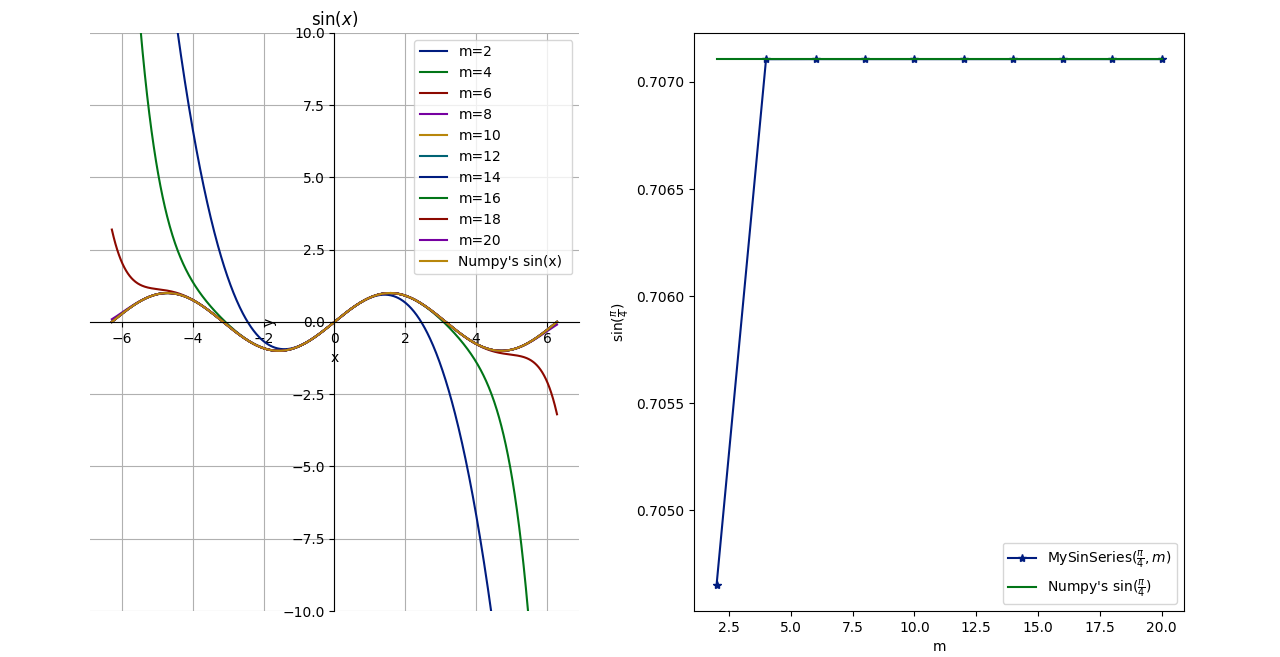
\includegraphics[width=\linewidth]{graph1}
	\caption[Graphs generated for MySinSeries]{Graphs generated for MySinSeries: The graph on the left shows the different taylor series approximations corresponding to different values of m=2,4,...20. The graph on the right shows how the value of $\sin(\pi/4)$ varies with different values of m.}
	\label{fig:graph1}
\end{figure}
\begin{figure}[H]
	\centering
	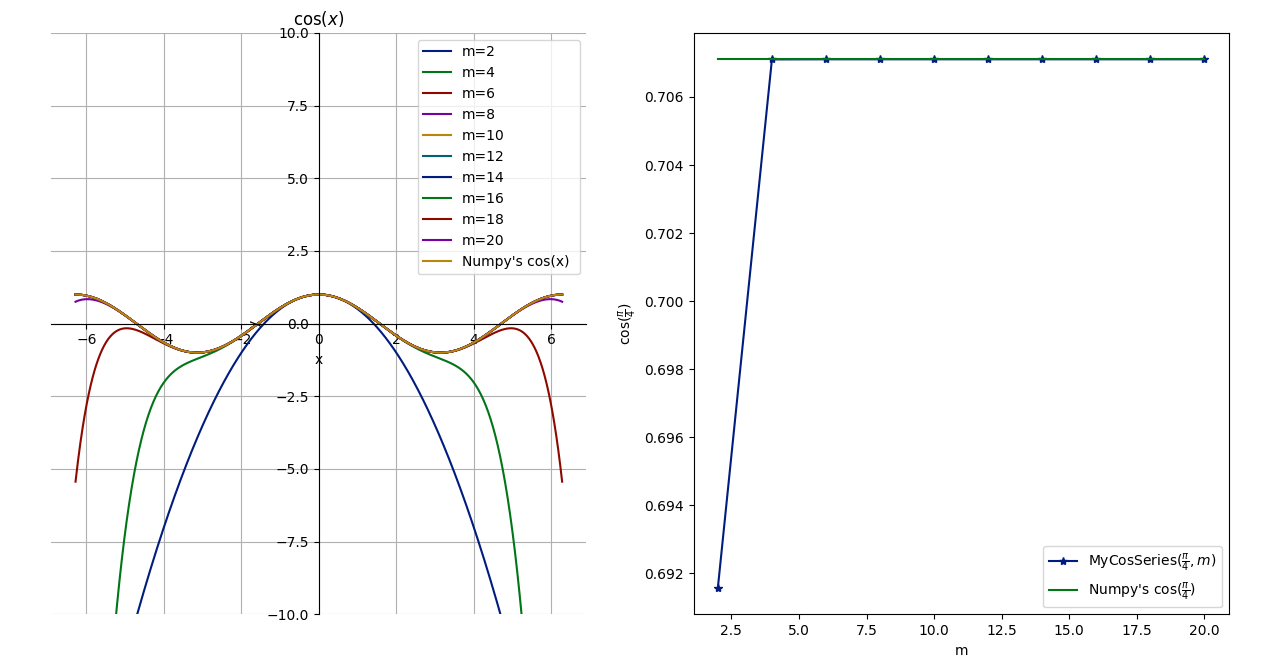
\includegraphics[width=\linewidth]{graph2}
	\caption[Graphs generated for MySinSeries]{Graphs generated for MySinSeries: The graph on the left shows the different taylor series approximations corresponding to different values of m=2,4,...20. The graph on the right shows how the value of $\sin(\pi/4)$ varies with different values of m.}
	\label{fig:graph2}
\end{figure}
\begin{figure}[H]
	\centering
	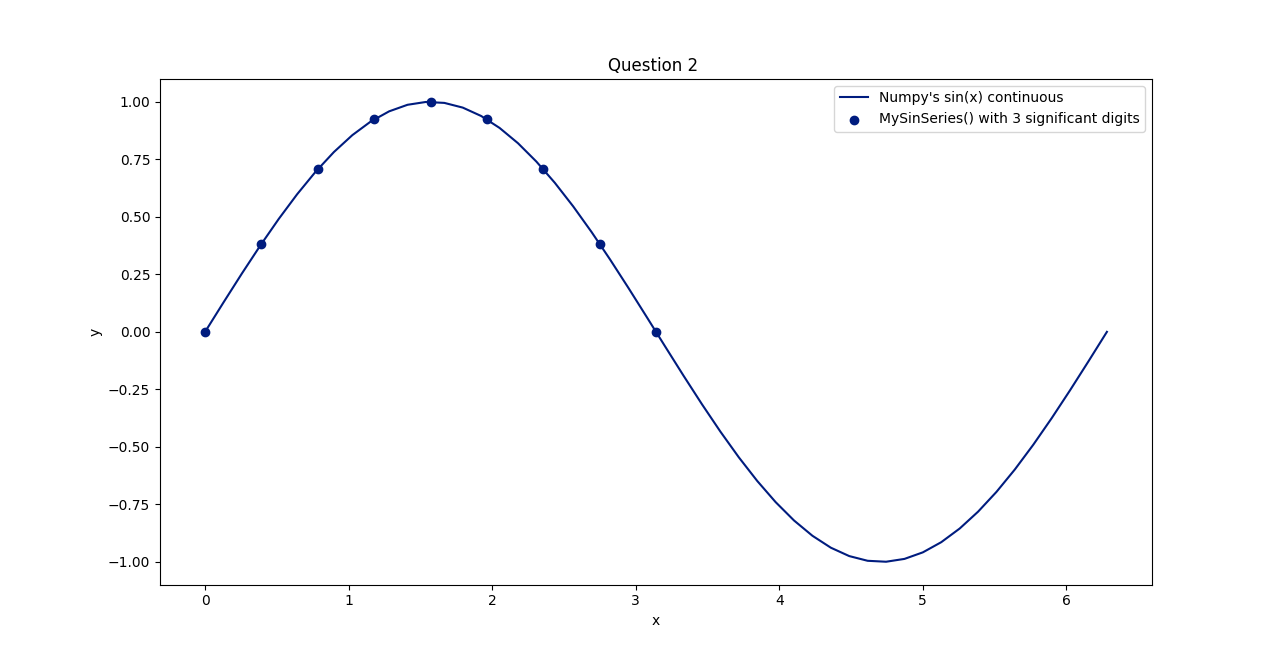
\includegraphics[width=0.7\linewidth]{graph3}
	\caption[Graphs generated for MySinSeries]{Graphs generated for MySinSeries: The graph on the left shows the different taylor series approximations corresponding to different values of m=2,4,...20. The graph on the right shows how the value of $\sin(\pi/4)$ varies with different values of m.}
	\label{fig:graph3}
\end{figure}

\end{document}
